\section{Descrizione generale}

\subsection{Obiettivi del prodotto}
\textit{Etherless} è un servizio sviluppato con una architettura decentralizzata\glo che permette agli sviluppatori di caricare funzioni JavaScript\glo sul cloud\glo per poi renderle disponibili ad utenti terzi (utilizzatori). Il servizio si presenta come un CaaS\glos (Computation-as-a-Service) in cui l’utilizzatore paga per la singola esecuzione di una funzione in modo automatico mediante l’utilizzo della rete Ethereum\glo e degli smart contract\glo. Una parte del compenso verrà accreditata allo sviluppatore mentre, la restante, verrà trattenuta da \textit{Etherless}.

\subsection{Funzioni del prodotto}
L'obbiettivo finale è quello di avere un ambiente in cui un ipotetico sviluppatore \textit{Bob}, dopo aver creato una funzionalità che potrebbe essere di interesse per altri sviluppatori (es. \textit{Alice}), carica il suo codice JavaScript su \textit{Etherless} mediante la sua utenza e ne imposta un costo di esecuzione. \textit{Alice}, abile programmatrice, avendo bisogno di tale funzionalità, può pagare la quota di esecuzione piuttosto che riscrivere la stessa procedura; attraverso la sua utenza \textit{Etherless}, \textit{Alice} può dunque usufruire della funzione in cloud pagandone il costo di esecuzione ad ogni singola chiamata.
\\\\
Ogni utente del servizio viene rappresentato da un account Ethereum\glo, identificato da un indirizzo e da una chiave privata. Possiamo fare una distinzione logica tra:
\begin{itemize}
	\item \textbf{Utente utlizzatore} colui che decide di utilizzare funzioni altrui.
	\item \textbf{Utente sviluppatore}: colui che decide di rendere pubblica una o più funzioni;
	\item \textbf{Utente generico} utente che non si è autenticato nella rete Ethereum\glo.
\end{itemize} 
l'\textbf{utente utlizzatore} può:
\begin{itemize}
	\item elencare tutte le funzioni disponibili;
	\item eseguire una funzione tra le disponibili;
	\item effettuare il logout della sua utenza.
\end{itemize}
l'\textbf{utente sviluppatore}, oltre che effettuare le stesse operazioni rese disponibili agli utenti utilizzatori, può:
\begin{itemize}
	\item elencare le funzioni da lui rese pubbliche;
	\item creare una nuova funzione e specificarne nome e costo di esecuzione;
	\item caricare il codice relativo ad una sua funzione;
	\item eliminare una funzione da lui pubblicata;
	\item visualizzare il log delle chiamate alle sue funzioni.
\end{itemize}
Un \textbf{utente generico} può:
\begin{itemize}
	\item registrarsi al servizio richiedendo un nuovo account;
	\item accedere alla sua utenza inserendo le credenziali di accesso;
\end{itemize}


\subsection{Caratteristiche}
\subsubsection{Caratterische utenti}
\subsubsection{Identificazione}
Gli utenti \textit{Etherless} sono identificati univocamente attraverso un account Ethereum\glos. Questo significa che un account utente non è identificato e caratterizzato da parametri ``comuni'' (come ad esempio nome, cognome, email, password, etc.) ma da una combinazione di \textit{address} e \textit{private-key}\glo specifici delle reti blockchain\glo.
\subsubsection{Autenticazione}
Per la persistenza della sessione dell'utente, verranno salvati nel file system\glo del computer le credenziali di accesso in seguito alla registrazione o all'accesso dell'utente su una istanza dell'\textit{Etherless-cli}. In particolar modo, un utente generico potrà effettuare le seguenti operazioni:
\begin{itemize}
	\item \textbf{Accesso}: nel caso l'utente voglia accedere alla sua utenza \textit{Etherless}, gli verrà chiesto di inserire le sue credenziali;
	\item \textbf{Registrazione}: nel caso della registrazione di una nuova utenza, verrà inoltrata la richiesta alla rete Ethereum\glo che genererà un combinazione di credenziali univoca.
\end{itemize}
\subsubsection{Crediti}
Ogni utente ha associato al suo account un certo numero di Ether\glo. Non è stato richiesto di prevedere una modalità di ricarica di tali crediti. Ogni account, alla sua creazione, avrà a disposizione un certo numero di Ether\glo.

\subsection{Caratteristiche tecniche}
La piattaforma deve essere conforme a quanto segue:
\begin{itemize}
	\item gli utenti avranno la possibilità elencare le funzioni disponibili,  caricarne di nuove, aggiornarle, eseguirle oppure eliminare attraverso \textit{Etherless-cli};
	\item sarà utilizzata la rete \textit{Ethereum}\glo per la comunicazione tra i vari componenti di \textit{Etherless}, per la definizione della logica di interazione tra le varie parti (smart contract\glos) e per lo storage\glo di dati;
	\item per la realizzazione del back-end\glo deve essere prevista una infrastruttura Serverless\glo;
	\item Utilizzo del servizio AWS Lambda per lo storage\glo ed esecuzione in cloud\glo delle funzioni caricate;
	\item La comunicazione tra i vari componenti di \textit{Etherless} deve avvenire solamente attraverso eventi Ethereum\glo; TODOOOOOO INSERIREI LA LORO IMMAGINEEE

\end{itemize}
L'intero sistema si basa su tre applicativi software:
	\begin{itemize}
		\item \textbf{\textit{Etherless-cli:}} CLI\glo attraverso la quale gli utenti si interfacciano con il servizio ed eseguono le funzionalità disponibili;
		\item \textbf{\textit{Etherless-smart:}} applicativo che si occupa della definizione e del deploy\glo dello smart contract sulla rete Ethereum\glos;
		\item \textbf{\textit{Etherless-server:}} applicativo server che rimane in ascolto e soddisfa le richieste di esecuzione delle funzioni caricate, interfacciandosi con il servizio AWS Lambda mediante l'apposito SDK\glos;
	\end{itemize}
\subsubsection{Trasferimento del denaro}
Ogni qualvolta venga utilizzata una delle funzioni messe a disposizione dagli utenti sviluppatori, deve avvenire il corrispettivo pagamento da parte dell'utilizzatore. Sono state individuate due possibili modalità di trasferimento del denaro:
\begin{itemize}
	\item trasferimento diretto dei fondi quando lo smart-contract\glo riceve la richiesta di esecuzione;
	\item mediante escrow\glos, i soldi vengono prelevati dall'utilizzatore alla ricezione della richiesta di esecuzione e accreditati allo sviluppatore solamente quando l'output della funzione richiesta raggiunge l'utilizzatore.
\end{itemize}
Il proponente \textit{Red Babel} ha specificato che la prima versione è accettata.

\subsubsection{Archiviazione dei dati}
Per lo storage dei dati non è previsto l'utilizzo di database. Dalle specifiche del capitolato\glo emerge che non è necessario il salvataggio di dati quali immagini o descrizioni. Informazioni come nomi di funzioni, ownership\glo e costi di esecuzioni verranno salvati direttamente sulla rete Ethereum\glo attraverso lo smart contract\glos; 
\\\\
Nel caso in cui sorga la necessità di salvare quantitativi più grandi di dati, verrà utilizzato un database relazionale o non-relazionale disponibile tramite AWS;
\subsubsection{Accesso alle risorse}
\begin{itemize}
	\item L'utente in generale ha accesso a tutte le funzioni pubblicate vedendone il nome, i parametri richiesti, e richiederne l'esecuzione;
	\item Lo sviluppatore, sulle funzioni di sua proprietà, può vederne il nome e parametri associati, caricare e modificare il codice, eliminare una funzione e crearne di nuove;
	\item Alle risorse disponibili su AWS hanno accesso solo \textit{Etherless-cli} e \textit{Etherless-server};
\end{itemize}
\subsubsection{Tecnologie}
Le tecnologie da utilizzare per la realizzazione del prodotto sono:
\begin{itemize}
	\item \textbf{AWS (Amazon Web Services)}: piattaforma che si occupa di fornire servizi di cloud computing\glos;
	\item \textbf{AWS - Lambda}: servizio che consente di eseguire codice nel cloud\glos;
	\item \textbf{Ethereum}: una rete globale per il trasferimento di criptovalute\glo e per la realizzazione di applicativi decentralizzati;
	\item \textbf{Solidity}: linguaggio OOP\glo per la definizione di smart contract\glos;
	\item \textbf{Truffle}: framework per lo sviluppo di smart contract\glo su rete Ethereum\glo;
	\item \textbf{Web3}: API\glo JavaScript per l'interazione con un nodo Ethereum\glo locale o remoto;
	\item \textbf{Ropsten}: Rete Ethereum\glo pubblica usata per il testing di applicativi Ethereum\glo in ambiente di staging;
	\item \textbf{MainNet}: Rete Ethereum\glo principale;
	\item \textbf{Ganache}: Ambiente di sviluppo Ethereum\glo utilizzato per la simulazione locale;
	\item \textbf{TypeScript 3.6}:  linguaggio open-source\glo sviluppato da Microsoft che estende le potenzialità di Javascript;
	\item \textbf{Node.js}: ambiente di runtime\glo open-source\glo per JavaScript;
	\item \textbf{The Serverless Framework}: framework\glo per la costruzione e deploy\glo  di ambienti serverless\glos;
	\item \textbf{Smart Contract}: protocollo informatico che facilita, verifica, fa rispettare ed esegue un contratto;
	\item \textbf{ESLint}: strumento di analisi statica del codice JavaScript;
\end{itemize}
\subsection{Ambienti}
Il cliente ha richiesto la possibilità di eseguire il programma nelle seguenti modalità:
\begin{itemize}
	\item \textbf{Locale:} simulando una rete Ethereum\glo sulla propria macchina;
	\item \textbf{Test:} simulando una rete Ethereum\glo su un ambiente di test condiviso tra gli sviluppatori del progetto;
	\item \textbf{Staging:} utlizzando un rete Ethreum\glo di test pubblica come Ropsten\glos;
	\item \textbf{Production:} utilizzando la rete Ethereum\glo ufficiale MainNet\glos.
\end{itemize}
A tale scopo deve essere prevista la configurazione dei vari ambienti su \textit{Etherless-smart}, \textit{Etherless-cli} e \textit{Etherless-server}.
\subsection{Architetture del progetto}
Come già anticipato, le componenti necessarie per la realizzazione di \textit{Etherless} sono \textit{Etherless-cli, Etherless-smart} e \textit{Etherless-server}. L'architettura del servizio sarà quella di una applicazione decentralizzata\glo (DApp\glo) basandosi su una rete di computer Peer-to-Peer\glo e sfruttando la tecnologia blockchain\glo.\\
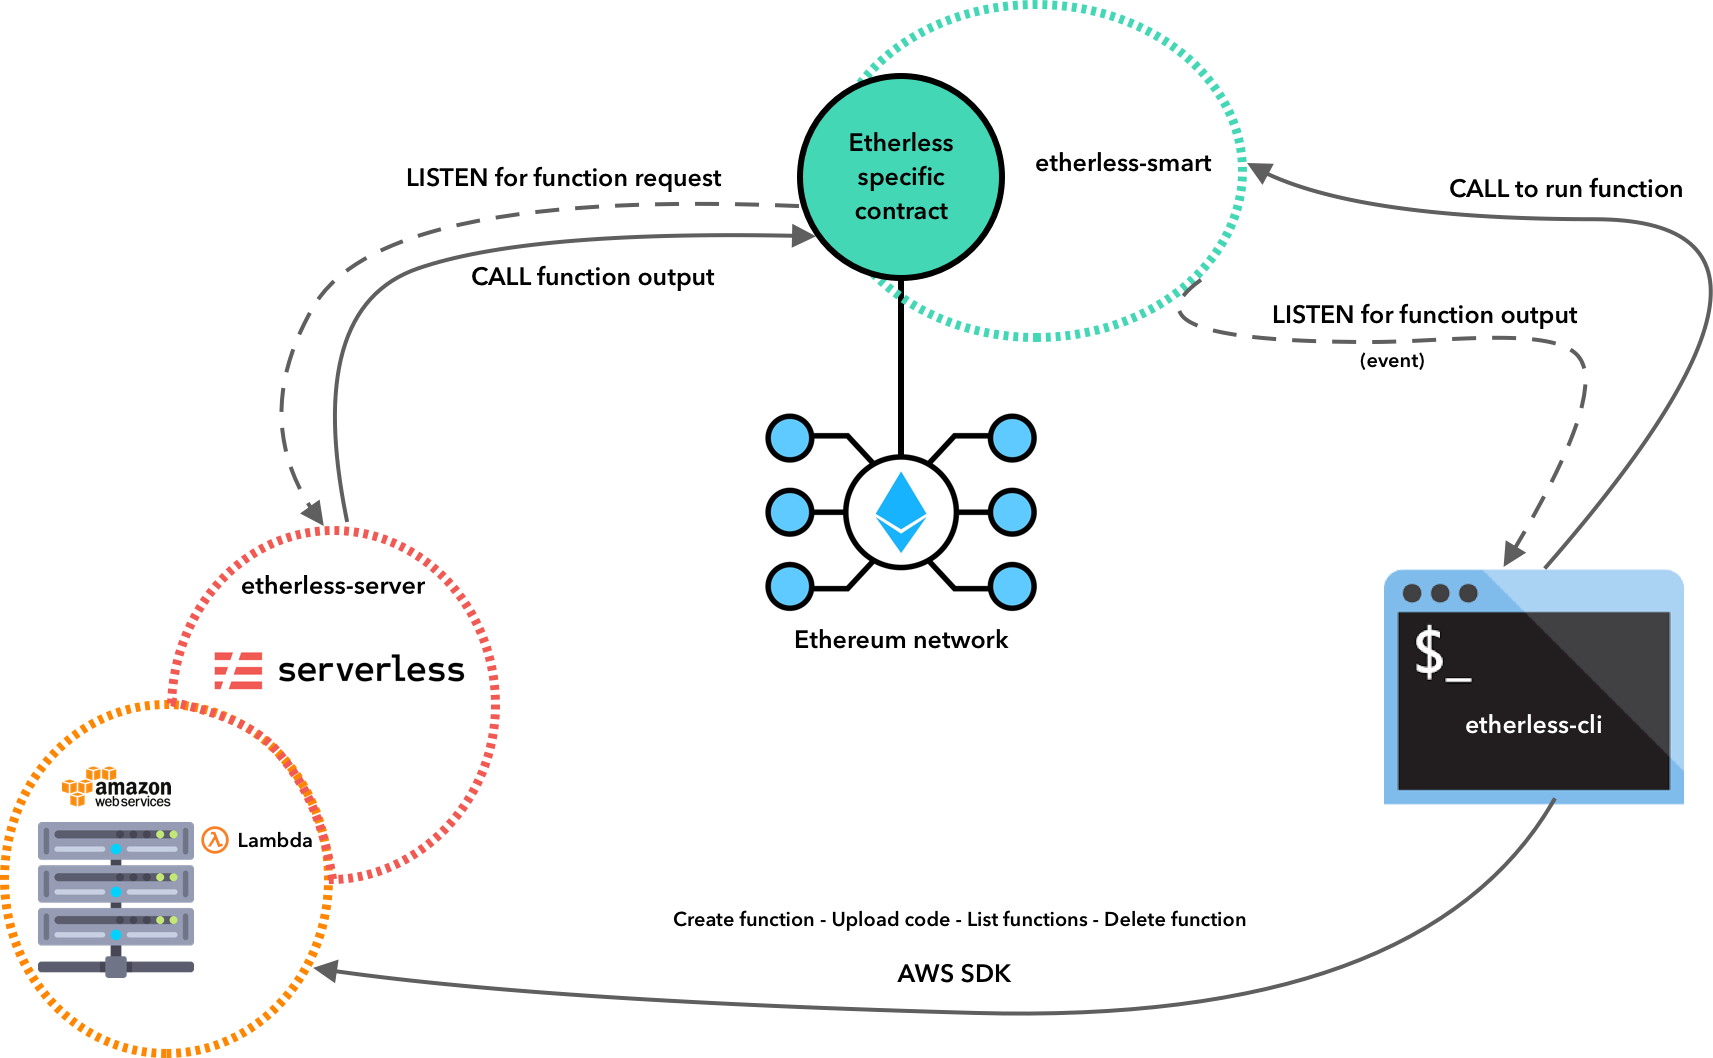
\includegraphics[width=\textwidth]{res/img/archi}
\subsubsection{Etherum\glo network}
Il servizio si baserà sull'utilizzo degli smart-contract\glos, che si occuperanno di regolare indirettamente le interazioni tra sviluppatori e, in modo diretto, l'esecuzione delle funzioni e l'interazione tra l'utente utilizzatore e il servizio. Inoltre, lo smart-contract\glos, sarà utilizzato come storage per i dati dell'applicazione. Una volta definite le regole del contratto, questo viene reso pubblico mediante la sua compilazione e deploy\glo sul network Ethereum\glos. Tale operazione permetterà di ottenere un indirizzo e un ABI\glo del rispettivo contratto nella rete Ethereum\glos. Questi dati saranno utili a \textit{Etherless-cli} e \textit{Etherless-server} per potersi interfacciare il contratto.
\subsubsection{Front-end}
L'interazione tra l'utente e il servizio avviene attraverso una CLI\glo che prende il nome di \textit{Etherless-cli}. L'utilizzo è di tipo richiesta-risposta: l'utente avvia \textit{Etherless-cli} e, digitando un comando specifico, l'applicativo ricava l'output corrispondente mostrandolo a video. \\Per completare la richiesta dell'utente, il processo può richiamare funzioni del contratto oppure mettersi in ascolto di eventi sulla rete Ethereum\glos.
\\Nel caso in cui l'utente sia uno sviluppatore e venga richiesto l'upload di una nuova funzione, questo componente, tramite l'SDK\glo di AWS, caricherà la funzione su AWS Lambda\glos.
\subsubsection{Serverless}
\textit{Etherless-server} è un processo che verrà messo in esecuzione continua sfruttando il framework Serverless e impostando AWS come destinazione del deploy\glos.\\
Quando lo smart-contract\glo riceve una richiesta di esecuzione di una funzione remota, viene emesso un evento che specifica il nome e i parametri con i quali eseguirla. \textit{Etherless-server}, messo in ascolto per questa tipologia di eventi, utilizzerà l'SDK\glo di AWS per ottenere il risultato dell'esecuzione della funzione e restituirla a \textit{Etherless-cli}.

\subsubsection{Schema di interazione}
Di seguito viene mostrato quale deve essere il flusso delle interazioni dei vari componenti.\\
	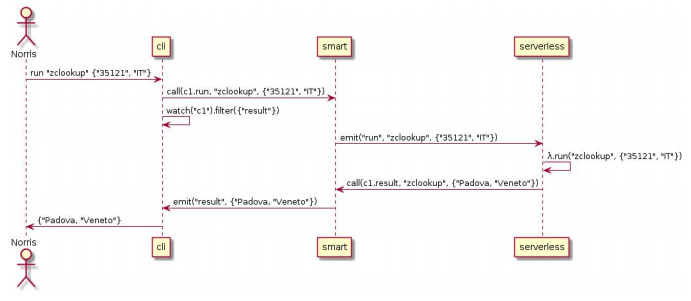
\includegraphics[width=\textwidth]{res/img/calls-flow}
\subsection{Vincoli del sistema}
\subsubsection{Per l'utente}
Per l'esecuzione è necessaria una connessione ad Internet, l'installazione di Node.js, e il download di \textit{Etherless-cli}. Per accedere al servizio l'utente dovrà prima creare una utenza oppure accedere con una già esistente. Preferibilmente richieste conoscenze nell' utilizzo della CLI\glo.
\subsubsection{Per il servizio}
Per l'esecuzione serverless\glo del servizio è richiesta una utenza AWS e la corretta configurazione di tale ambiente. Inoltre, è necessario poter accedere a un network Ethereum\glo.
	
	